% RECOMMENDED %%%%%%%%%%%%%%%%%%%%%%%%%%%%%%%%%%%%%%%%%%%%%%%%%%%
\documentclass[graybox]{svmult}

% choose options for [] as required from the list
% in the Reference Guide

\usepackage{mathptmx}       % selects Times Roman as basic font
\usepackage{helvet}         % selects Helvetica as sans-serif font
\usepackage{courier}        % selects Courier as typewriter font
\usepackage{type1cm}        % activate if the above 3 fonts are
                            % not available on your system
%
\usepackage{makeidx}         % allows index generation
\usepackage{graphicx}        % standard LaTeX graphics tool
                             % when including figure files
\usepackage{multicol}        % used for the two-column index
\usepackage[bottom]{footmisc}% places footnotes at page bottom
\usepackage{tabularx}
\usepackage{booktabs}
\usepackage{pdflscape}
\usepackage{url}
\urlstyle{same}

\usepackage[numbers,sort]{natbib} % "sort" = "orders multiple citations into the sequence in which they 
% appear in the list of references;"
%\usepackage[style=numeric,sorting=none,natbib=true,backend=biber]{biblatex}

% see the list of further useful packages
% in the Reference Guide


\makeindex             % used for the subject index
                       % please use the style svind.ist with
                       % your makeindex program


% fix table columns
\newcolumntype{Y}{>{\centering\arraybackslash}X}

%%%%%%%%%%%%%%%%%%%%%%%%%%%%%%%%%%%%%%%%%%%%%%%%%%%%%%%%%%%%%%%%%%%%%%%%%%%%%%%%%%%%%%%%%

\begin{document}

\title*{Incorporating emotion and personality-based analysis in user-centered modelling}
% Use \titlerunning{Short Title} for an abbreviated version of
% your contribution title if the original one is too long
\author{Mohamed Mostafa \and Tom Crick \and Ana C. Calderon \and Giles Oatley}
% Use \authorrunning{Short Title} for an abbreviated version of
% your contribution title if the original one is too long
\institute{Mohamed Mostafa \and Tom Crick \and Ana C. Calderon \at
  Department of Computing \& Information Systems, Cardiff Metropolitan
  University, Cardiff, UK;
  \email{{momostafa,tcrick,acalderon}@cardiffmet.ac.uk}
\and
Giles Oatley \at School of Engineering \& Information Technology,
Murdoch University, Australia;\\\email{g.oatley@murdoch.edu.au}}
%
% Use the package "url.sty" to avoid
% problems with special characters
% used in your e-mail or web address
%
\maketitle

\abstract{Understanding user behaviour under varying conditions,
scenarios and journeys is fundamental to the improvement of the
user-experience for a given system. Predictive models of user
reactions and responses can aid in the design of more intuitive and
usable systems. The research presented in this paper correlates events
and interactions in an online social network against user behaviour,
focusing on personality traits. Emotional context and tone is analysed
and modelled based on varying types of sentiments that users express
in their language using the IBM Watson Developer Cloud tools. The data
collected in this study thus provides further significant evidence
towards supporting the hypothesis that analysing and modelling
emotions, sentiments and personality traits provides valuable insight
into improving the user experience of complex social computer
systems.}

% Keywords: emotions; human computer interactions; social media;
% artificial intelligence; social analysis; affective computing.


\section{Introduction}\label{intro}

As computer systems and applications have become more widespread and
complex, with increasing demands and expectations of ever-more
intuitive human-computer interactions, research in modelling,
understanding and predicting user behaviour demands has become a
priority across a number of domains.  In these application domains, it
is useful to obtain knowledge about user profiles or models of
software applications, including intelligent agents, adaptive systems,
intelligent tutoring systems, recommender systems, e-commerce
applications and knowledge management
systems~\cite{schiaffino+amandi:2009}. Furthermore, understanding user
behaviour during system events leads to a better informed predictive
model capability, allowing the construction of more intuitive
interfaces and an improved user experience. This work can be applied
across a range of socio-technical systems, impacting upon both
personal and business computing.

We are particularly interested in the relationship between digital
footprint and behaviour and
personality~\citep{oatley+crick:2014,oatley-et-al_dasc2015,blamey-et-al-2012,blamey-et-al-2013}. A
wide range of pervasive and often publicly available datasets
encompassing digital footprints, such as social media activity, can be
used to infer
personality~\citep{lambiotte+kosinski:2014,oatley-et-al-soccogcomp2015}. Big
social data offers the potential for new insights into human behaviour
and development of robust models capable of describing individuals and
societies~\citep{lazer-et-al:2009}. Social media has been used in
varying computer system approaches; in the past this has mainly been
the textual information contained in blogs, status posts and photo
comments~\cite{blamey-et-al-2012,blamey-et-al-2013}, but there is also
a wealth of information in the other ways of interacting with online
artefacts. From sharing and gathering of information and data, to
catering for marketing and business needs; it is now widely used as
technical support for computer system platforms.

% according to a survey in 2009~\citep{thompson:2009}, more than 60\%,
% agrees with the statement that social media have been used as a
% technical support for posting technical issues for computer system.

% Academic research in image or
% video analysis includes promising studies on YouTube videos for
% classification of specific behaviours and indicators of personality
% traits~\citep{biel+gatica-perez:2012}. This work uses crowdsourced
% impressions, social attention, and audiovisual behavioural analysis on
% slices of conversational video blogs extracted from YouTube.

% \begin{figure}[!ht]
% \centering
% 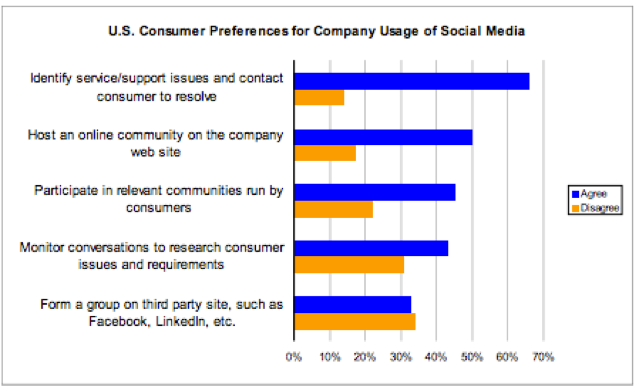
\includegraphics[width=\columnwidth]{images/socialmediause}
% \caption{US consumer preferences for company usage of social media~\citep{thompson:2009}}
% \label{fig:socialmediause} 
% \end{figure}
% (see Figure~\ref{fig:socialmediause}

The work presented in this paper is building upon previous work in
psycholinguistic science (the study of the psychological and
neurobiological factors that enable humans to acquire, use, comprehend
and produce language) and aims to provide further insight into how the
words and constructs we use in our daily life and online interactions
reflect our personalities and our underlying emotions. As part of this
active research field, it is widely accepted that written text
reflects more than the words and syntactic constructs, but also
conveys emotion and personality
traits~\citep{pennebaker+king:1999}. As part of our work, the IBM
Watson Tone Analyzer (part of the IBM Watson Developer Cloud
toolchain) has been used to identify emotion tones in the textual
interactions in an online system, building on previous work in this
area that shows a strong correlation between the word choice and
personality, emotions, attitude and cognitive processes, providing
further evidence that it is possible to profile and potentially
predict users’ identity~\citep{fast+funder:2008}. The
{\emph{Linguistic Inquiry and Word Count}} (LIWC) psycholinguistics
dictionary~\citep{pennebaker-et-al:2001,tausczik+pennebaker:2010} is
used to find psychologically meaningful word categories from word
usage in writing; the work presented here provides a modelling and
analysis framework, as well as associated toolchain, for further
application to larger datasets to support the research goal of
improving user-centered modelling.


\section{Personality Insight}\label{personality}

Numerous studies have suggested key words and phrases can signal
underlying tendencies and that this can form the basis of identifying
certain aspects of
personality~\citep{iacobelli-et-al:2011,pennebaker+king:1999,oberlander+gill:2004,oberlander+gill:2006}.
\citet{scherer:1984} introduced a valuable classification with the
following distinctions between emotions, moods, interpersonal stances,
attitudes and personality traits.

% \begin{itemize}
% \item {\emph{Emotion:}} short-lived, for instance being angry, sad, or joyful;
% \item {\emph{Mood:}} longer-lived, low-intensity for instance being cheerful or gloomy;
% \item {\emph{Interpersonal stances:}} duration linked to specific
%   interaction, for instance friendly or supportive;
% \item {\emph{Attitudes:}} long-lived linked to specific people or
%   events, for instance loving and hating;
% \item {\emph{Personality traits:}} stable personality dispositions and
%   typical behaviour tendencies, for instance nervous, anxious, or hostile.
% \end{itemize}

By observing the occurrences of words that related to these five
categories, we can conclude to certain degrees about the holder's
psychological state. For instance, we have sentiment analysis or
opinion mining at one end of the spectrum, by utilising open-source
software such as {\emph{SentiWordNet}}; at the other end of the
spectrum we have \citet{mairesse-et-al:2007} highlighting the use of
features from psycholinguistic databases such as
{\emph{LIWC}}~\citep{pennebaker-et-al:2001} to create a range of
statistical models for each of the Five Factor personality
traits. This ``Big Five'' model, focuses on five dimensions, namely:
{\emph{Agreeableness}}, {\emph{Conscientiousness}},
{\emph{Extraversion}}, {\emph{Neuroticism}} and
{\emph{Openness}}e~\citep{norman:1963,peabody+goldberg:1989}. It
should be noted that while researchers have continued to work with the
Five Factors model, there are well known
limitations~\cite{eysenck:1992,paunonen+jackson:2000,block:2010} that
are often overlooked; however, over the past 50 years the Five Factor
model has become a standard in psychology~\cite{mairesse-et-al:2007},
developing a large body of research for comparison.

% \begin{itemize}
% \item {\emph{Agreeableness}} is a person's inclination to be humane
%   and helpful toward others;
% \item {\emph{Conscientiousness}} is a person's being welling to the
%   tasks well and in an efficient organised way;
% \item {\emph{Extraversion}} is a person's level of socialisation and
%   enjoyment of being around people, the higher value means sociable
%   person, lower value means person's rather to be alone;
% \item {\emph{Neuroticism}} is a person's level to express some
%   negative emotions such as anger and stress.
% \item {\emph{Openness}} is the measurement of person's level to try
%   new things, adventure, imagination.
% \end{itemize}

%\subsection{Emotion Tones}

The IBM Watson Tone
Analyzer\footnote{\url{http://www.ibm.com/watson/developercloud/tone-analyzer.html}}
is a cloud-based framework to infer emotions from a given text; it
uses linguistic analysis to detect three types of tones from written
text: emotions, social tendencies, and writing style. Emotions
identified include {\emph{Anger}}, {\emph{Fear}}, {\emph{Joy}},
{\emph{Sadness}} and {\emph{Disgust}}; identified social tendencies
include the Big Five personality traits (as described above);
identified writing styles include {\emph{Confident}},
{\emph{Analytical}} and {\emph{Tentative}}. To derive emotion scores
from text, IBM Watson Tone Analyzer uses a stacked
generalisation-based ensemble framework to achieve greater predictive
accuracy~\citep{costa+mccrae:1992}.  Features such as n-grams
(unigrams, bigrams and trigrams), punctuation, emoticons, curse words,
greeting words (such as ``{\emph{hello}}'', ``{\emph{hi}}'' and
``{\emph{thanks}}'') and sentiment polarity are fed into machine
learning algorithms to classify emotion
categories~\citep{fellbaum:2006}. LIWC is used to find psychologically
meaningful word categories from word usage in writing.

IBM Watson Personality
Insights\footnote{\url{http://www.ibm.com/watson/developercloud/personality-insights.html}}
provides a deeper understanding of people's personality
characteristics, needs, and values to drive personalisation. It
extracts and analyses a spectrum of personality attributes to help
discover actionable insights about people and entities; the service
outputs personality characteristics that are divided into three
dimensions: the Big Five, {\emph{Values}} and {\emph{Needs}}. While
some services are contextually specific depending on the domain model
and content, Personality Insights usually only requires a minimum of
3500+ words of any text.


\section{Data Analysis \& Feature Extraction}

\subsection{Overview of the Data}

Our dataset comes from an online portal for a European Union (EU)
international scholarship mobility hosted at a UK university. The
dataset was generated from interactions between users and a complex
online information system, namely the online portal for submitting
applications.

The whole dataset consists of users (n=391), interactions and comments
(n=1390) as responses to system status and reporting their experience
with using the system. Google Analytics is used to track user behaviour
and web statistics (such as impressions); this data from has been used
to identify the server's status and categorised the status as two
stages: {\emph{Idle}, where the system had a higher number of active
sessions; and marked as {\emph{Failure}}, where the system had a lower
number of sessions engaged. Figure~\ref{fig:googleanalytics} provides
am example plot of web traffic from Google Analytics over one day, clearly
showing the drop at 20:00 where the system had been identified as in
the {\emph{Failure}} state.

\begin{figure}[!ht]
\centering
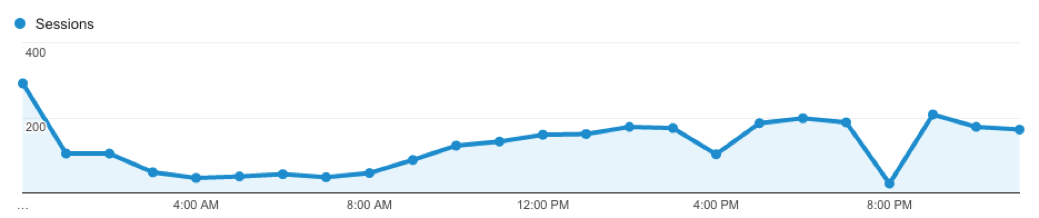
\includegraphics[width=\columnwidth]{images/googleanalytics}
\caption{Google Analytics profile shows behaviour of the system over a
  24 hour period (timeline during the day vs. number of active sessions)}
\label{fig:googleanalytics} 
\end{figure}

All interactions had been collected and grouped by server status, then
sent to the IBM Watson Tone Analyzer to generate the emotion social
tone scores, to provide an overview of the system behaviour and user’s
interaction with Facebook at the same
time. Figure~\ref{fig:emotiontone} shows the relationship between the
server behaviour and emotions of the users; in the system,
{\emph{Failure}} status shows a significant difference in overall
{\emph{Anger}} in different status; furthermore, the {\emph{Joy}}
parameter shows a significant difference with the system in
{\emph{Idle}} and {\emph{failure}} status. However {\emph{Fear}} and
{\emph{Sadness}} parameters is almost the same, even with the system in
{\emph{Idle}} status.

\begin{figure}[!ht]
\centering
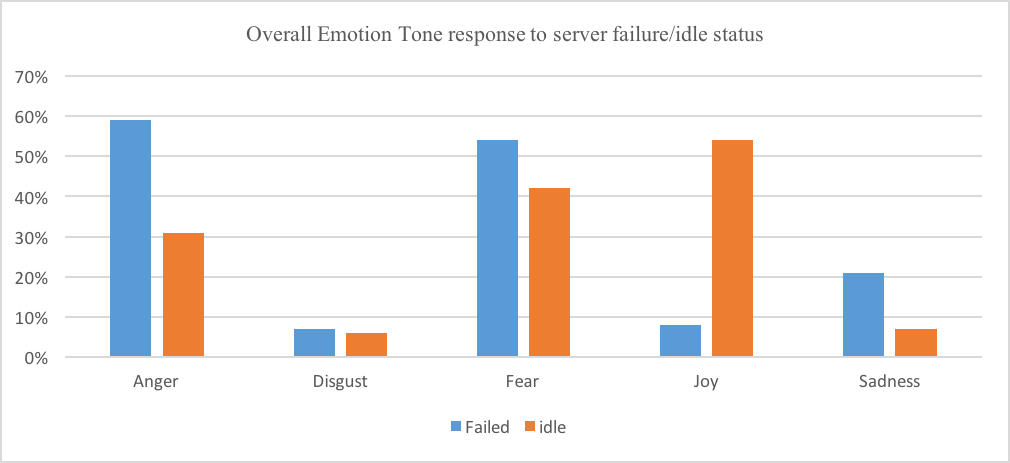
\includegraphics[width=\columnwidth]{images/emotiontone}
\caption{Overall emotion tone response to server failure/idle status}
\label{fig:emotiontone} 
\end{figure}

We identified the user's personality based on analysis of their
Facebook interactions (by collecting all comments from user), again by
using the IBM Watson Personality Insights tool. However,
a number of users in the dataset had completed the Big Five
questionnaire (n=44); in these instances, their Big Five scores have
been used instead. The second stage involved grouping the comments
based on server status and segmenting these interactions by user; this
allowed us to investigate the impact of server status in the emotion
of the user and investigate the Big Five dimension as a constant
parameter. By investigating the relationship between personality trait
dimensions and the social emotion tones, we are able to find the
highest correlation to identify the key elements of the potential
model by applying linear regression and Pearson correlation. This will
allow building of a neural network multilayer perception using the
potential key elements with higher correlations.

The previous overview encourages further investigation to understand
the relationship between user's behaviour and complex computer system
behaviours. The data collected from the social media interactions have
been grouped by users and using the IBM Watson Personality Insights,
we were able to identify the Big Five personality traits for each
user. Using the IBM Watson Tone Analyzer, the data has been grouped by
user's comments and server status ({\emph{Failure}}, {\emph{Idle}}) to
identify social emotion tone for each user. Table~\ref{tab:sample}
shows a sample of data used in this analysis, with each row
representing a unique user, and each column represents the Big Five
traits, social emotion tones and server status.

\begin{table}[!ht]
\centering
\resizebox{\columnwidth}{!}{%
\begin{tabular}{@{}rrrrrrrrrrr@{}}
\toprule
\multicolumn{1}{c}{Openness} & \multicolumn{1}{c}{Conscientiousness} & \multicolumn{1}{c}{Extraversion} & \multicolumn{1}{c}{Agreeableness} & \multicolumn{1}{c}{Neuroticism} & \multicolumn{1}{c}{anger} & \multicolumn{1}{c}{disgust} & \multicolumn{1}{c}{fear} & \multicolumn{1}{c}{joy} & \multicolumn{1}{c}{sadness} & \multicolumn{1}{c}{Server  Status} \\ 
\midrule
0.528 & 0.523 & 0.537 & 0.653 & 0.511 & 0.217821 & 0.793375 & 0.501131 & 0.031477 & 0.284936 & Failure \\
0.252 & 0.063 & 0.037 & 0.266 & 0.989 & 0.542857 & 0.084615 & 0.178302 & 0.224453 & 0.264283 & Failure \\
0.817 & 0.571 & 0.157 & 0.012 & 0.401 & 0.162798 & 0.166694 & 0.213870 & 0.410916 & 0.220049 & Failure \\
0.197 & 0.130 & 0.180 & 0.419 & 0.990 & 0.468938 & 0.259794 & 0.350803 & 0.037265 & 0.636412 & Failure \\
0.155 & 0.079 & 0.081 & 0.226 & 0.975 & 0.539162 & 0.219993 & 0.431932 & 0.011625 & 0.642158 & Failure \\
0.158 & 0.281 & 0.332 & 0.510 & 0.869 & 0.419015 & 0.162022 & 0.213941 & 0.066892 & 0.686369 & Failure \\
0.817 & 0.571 & 0.157 & 0.012 & 0.401 & 0.041602 & 0.026298 & 0.141606 & 0.651962 & 0.106500 & Failure \\
0.058 & 0.038 & 0.147 & 0.375 & 0.989 & 0.449222 & 0.057946 & 0.181654 & 0.158412 & 0.547968 & Idle \\
0.178 & 0.138 & 0.800 & 0.564 & 0.828 & 0.207497 & 0.096643 & 0.093218 & 0.769316 & 0.162241 & Idle \\
0.105 & 0.463 & 0.792 & 0.704 & 0.041 & 0.134487 & 0.257145 & 0.195858 & 0.181699 & 0.509379 & Idle \\
0.589 & 0.479 & 0.147 & 0.339 & 0.828 & 0.360527 & 0.240875 & 0.321188 & 0.117492 & 0.212762 & Idle \\
0.338 & 0.235 & 0.104 & 0.304 & 0.869 & 0.164107 & 0.015058 & 0.230148 & 0.629562 & 0.356028 & Idle \\
0.204 & 0.203 & 0.480 & 0.329 & 0.892 & 0.625891 & 0.193692 & 0.242459 & 0.153679 & 0.166561 & Idle \\
0.689 & 0.968 & 0.805 & 0.465 & 0.029 & 0.246246 & 0.080353 & 0.123761 & 0.807537 & 0.135646 & Idle \\
0.093 & 0.175 & 0.642 & 0.563 & 0.875 & 0.279503 & 0.045658 & 0.207278 & 0.088724 & 0.505607 & Idle \\
0.277 & 0.296 & 0.276 & 0.332 & 0.892 & 0.499199 & 0.143897 & 0.269725 & 0.188664 & 0.285462 & Idle \\
0.055 & 0.095 & 0.783 & 0.699 & 0.935 & 0.450997 & 0.153940 & 0.263070 & 0.350778 & 0.116282 & Idle \\ 
\bottomrule
\end{tabular}%
}
\caption{Example data snapshot used in the analysis}
\label{tab:sample}
\end{table}

\subsection{Statistical Analysis}

As part of modelling the user's responsive behaviour, one of the
approaches to build a conceptual framework model is to apply linear
regression to investigate the relationship between the Big Five
personality dimensions and the emotion tones features.


\begin{figure}[!ht]
\centering
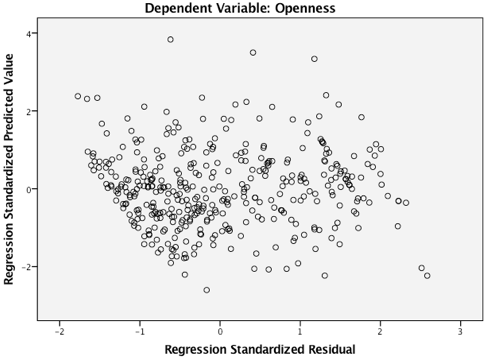
\includegraphics[width=0.45\columnwidth]{images/opennessplot.png}
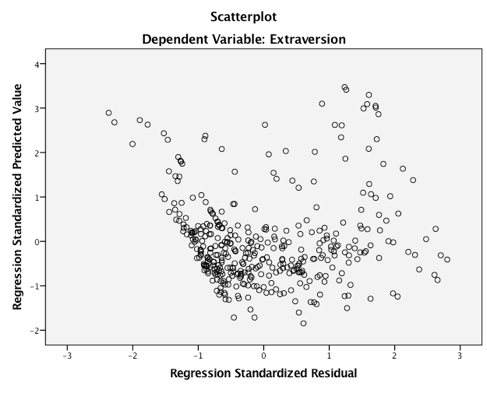
\includegraphics[width=0.45\columnwidth]{images/extraversionplot.png}\\
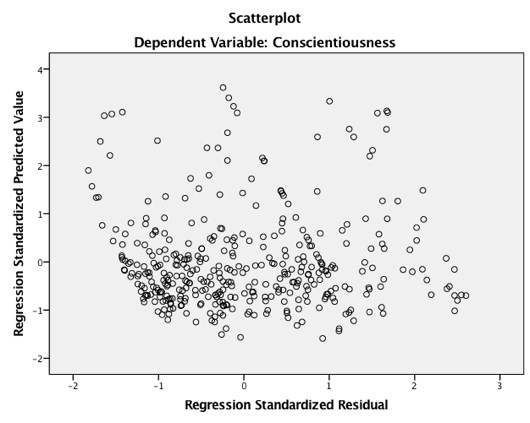
\includegraphics[width=0.45\columnwidth]{images/conscientiousnessplot.png}
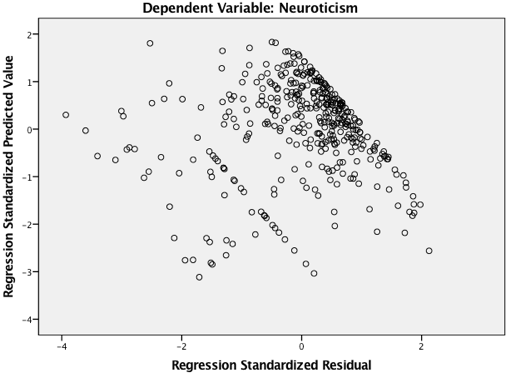
\includegraphics[width=0.45\columnwidth]{images/neuroticismplot.png}\\
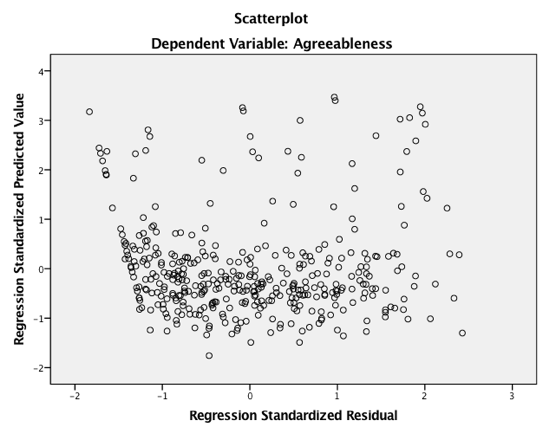
\includegraphics[width=0.45\columnwidth]{images/agreeablenessplot.png}
\caption{Scatterplots of Big Five dimension (dependent variables) and
  social emotion tones (independent variables)}
\label{fig:scatterplots} 
\end{figure}


\begin{table}[!ht]
\centering
\resizebox{\columnwidth}{!}{%

\begin{tabular}{@{}llll|lll|lll|lll|lll@{}}
%\begin{tabularx}{\textwidth}{llll|lll|lll|lll|lll}
\toprule
& \multicolumn{3}{c}{Openness} & \multicolumn{3}{c}{Extraversion} &
\multicolumn{3}{c}{Conscientiousness} &
\multicolumn{3}{c}{Agreeableness} & \multicolumn{3}{c}{Neuroticism} \\

\midrule
           
& \multicolumn{1}{c}{B} & \multicolumn{1}{c}{t} &
\multicolumn{1}{c}{Sig} & \multicolumn{1}{c}{B} &
\multicolumn{1}{c}{t} & \multicolumn{1}{c}{Sig} &
\multicolumn{1}{c}{B} & \multicolumn{1}{c}{t} &
\multicolumn{1}{c}{Sig} & \multicolumn{1}{c}{B} &
\multicolumn{1}{c}{t} & \multicolumn{1}{c}{Sig} &
\multicolumn{1}{c}{B} & \multicolumn{1}{c}{t} &
\multicolumn{1}{c}{Sig} \\


(constant) & 0.356                 & 3.282                 & 0.001                   & 0.162                 & 1.642                 & 0.101                   & 0.16                  & 1.623                 & 0.105                   & 0.297      & 2.831     & 0.005    & 0.828          & 9.934   & 0      \\
anger      & -0.063                & -0.735                & 0.463                   & 0.064                 & 0.831                 & 0.406                   & 0.124                 & 1.592                 & 0.112                   & 0.024      & 0.293     & 0.769    & 0.116          & 1.767    & 0.078     \\
disgust    & 0.478                 & 4.354                 & 0                       & 0.114                 & 1.142                 & 0.253                   & 0.255                 & 2.551                 & 0.011                   & -0.061     & -0.574    & 0.566    & -0.363         & -4.303    & 0    \\
fear       & 0.065                 & 0.534                 & 0.594                   & 0.172                 & 1.549                 & 0.122                   & 0.04                  & 0.356                 & 0.722                   & 0.093      & 0.783     & 0.434    & -0.023         & -0.241    & 0.81    \\
joy        & 0.066                 & 0.561                 & 0.575                   & 0.446                 & 4.179                 & 0                       & 0.436                 & 4.058                 & 0                       & 0.188      & 1.652     & 0.099    & -0.487         & -5.39   & 0      \\
sadness    & -0.226                & -2.118                & 0.035                   & -0.185                & -1.906                & 0.057                   & -0.03                 & -0.313                & 0.754                   & 0.014      & 0.132     & 0.895    & 0.233          & 2.841     & 0.005    \\

\bottomrule

%\end{tabularx} 
\end{tabular}%
}
\caption{Linear regression coefficients}
\label{tbl:linreg}
\end{table}

The linear regression (see Table~\ref{tbl:linreg} and
Figure~\ref{fig:scatterplots}) does not show significant correlations
between the Big Five dimensions and the social emotion tones; however,
certain correlations can be highlighted and used as key elements for
the model at this stage. The correlation of {\emph{Openness} and
{\emph{Disgust}}, is 0.479; the correlation of {\emph{Extraversion}}
and {\emph{Joy}} is 0.446 with p-value of
zero. {\emph{Conscientiousness}} and {\emph{Joy}} with 0.436
correlation and [\emph{Disgust}} with 0.255. {\emph{Agreeableness}},
does not appear to have a high impact in the social emotion
parameters, with the highest correlation being 0.188 with
{\emph{Joy}}, which can be overlooked as a useful factor in the
model. {\emph{Neuroticism}} and {\emph{Disgust} is -0.363, {\emph{Joy}
is -0.487 and p-value is zero is both cases; and {\emph{Sadness}} with
0.233. All correlation values are $<$0.5; however, it is noticed that
{\emph{Agreeableness}} does not have a linear relationship with any of
the social emotion tones. Furthermore, the social emotion tones that
have a potential linear relationship are {\emph{Disgust}},
{\emph{Joy}} and {\emph{Sadness}}, since the three tones have a
correlation between $>$0.3 and $<$0.5.

Previous linear regression analysis suggested that the following Big
Five dimensions ({\emph{Openness}}, {\emph{Extraversion}},
{\emph{Conscientiousness}} and {\emph{Neuroticism}}) have the highest
correlation with the social emotion tones ({\emph{Joy}},
{\emph{Sadness}} and {\emph{Disgust}}). For further analysis, the
Pearson correlation for the same dataset has been performed to compare
the output with the linear regression correlations. As you can see in
Table~\ref{tab:pearson}, there is no significant correlation in both;
however, in the Pearson correlation, {\emph{Neuroticism}} has the
highest correlation values across emotion tones, especially
{\emph{Anger}}, {\emph{Joy}} and {\emph{Sadness}}. {\emph{Joy}} does
have a correlation with all Big Five dimensions except for
{\emph{Agreeableness}} which agrees with the previous
analysis. However, {\emph{Disgust}} does not have a strong correlation
with any of the Big Five dimensions, which deviates from the previous
analysis.

\begin{table}[!ht]
\centering
\begin{tabular}{@{}rrrrrr@{}}
\toprule
                  & \multicolumn{1}{c}{Anger}  & \multicolumn{1}{c}{Disgust} & \multicolumn{1}{c}{Fear}   & \multicolumn{1}{c}{Joy}    & \multicolumn{1}{c}{Sadness} \\ 
\midrule
Openness          & -0.098 & 0.231   & 0.043  & 0.035  & -0.151  \\
Conscientiousness & -0.111 & -0.001  & -0.113 & 0.267  & -0.19   \\
Extraversion      & -0.175 & -0.077  & -0.071 & 0.349  & -0.291  \\
Agreeableness     & -0.068 & -0.089  & -0.027 & 0.14   & -0.069  \\
Neuroticism       & 0.375  & -0.037  & 0.153  & -0.488 & 0.379   \\ 

\bottomrule
\end{tabular}
\caption{Pearson correlations}
\label{tab:pearson}
\end{table}


\subsection{Key Elements of the Model}

According to the output of the statistical analysis presented in
Table~\ref{tbl:linreg} (linear regression) and Table~\ref{tab:pearson}
(Pearson correlation), the Big Five dimension identified as the key
elements from the personality traits are: {\emph{Openness}},
{\emph{Extraversion}}, {\emph{Conscientiousness}} and
{\emph{Neuroticism}}. The statistical analysis agrees that
{\emph{Agreeableness}} does not have a significant correlation across
any of the social emotion tones. The social emotion tones to be used
as key input elements for the proposed model are {\emph{Joy}},
{\emph{Sadness}}, {\emph{Anger}} and {\emph{Disgust}}; although the
{\emph{Anger}} tone did not show any significant correlation in linear
regression analysis, the value of the Pearson correlation coefficient
is between 0.3 and 0.5 which can be used as input for the model.

\begin{table}[!ht]
\centering
\begin{tabular}{lrr}
Correctly classified instances:   & 43     & ({\emph{75.44\%}}) \\
Incorrectly classified instances: & 14     & ({\emph{24.56\%}}) \\
Kappa statistic:                  & 0.5295 &         \\
Mean absolute error:              & 0.3432 &         \\
Root mean squared error:          & 0.4246 &         \\
Total number of instances:        & 57     &        
\end{tabular}
\caption{Re-evaluation output of proposed model}
\label{tab:reeval}
\end{table}

The dataset used to build this model is based upon a number of users
(n=391), eight inputs ({\emph{Openness}}, {\emph{Extraversion}},
{\emph{Conscientiousness}}, {\emph{Neuroticism}}, {\emph{Joy}},
{\emph{Sadness}}, {\emph{Anger}} and {\emph{Disgust}}) and the
class/output variable as the server status (where No: System
{\emph{Failure}} and Yes: System {\emph{Idle}}). As shown in
Table~\ref{tab:reeval}, the total number of the instances for the
testing set is 57. The output of the model shows a 75.44\% corrected
predicted instances and 24.56\% incorrectly classified instances. As
this has been performed on a small subset of the overall larger
project dataset, the output data is encouraging and provides the
infrastructure for further analysis and research to exploit the full
dataset.


\section{Conclusions and Future Work}\label{conclusions}

This paper presents preliminary results from a larger ongoing theme of
research to profile online/digital
behaviour~\citep{oatley+crick:2014,oatley-et-al_dasc2015}, which could
provide the conceptual framework to improve user experience and
computer system architecture design. Social media is now not only
being used as a content and sharing platform, but also as a platform
for technical support for various of online applications and
services. This paper demonstrates the analysis of one such online
application that has used Facebook as technical support platform for
the users. Such social networks provide substantial textual and
interaction datasets for analysis, providing further insight into
personality traits and social emotion tones.

We are also interested in profiling complex behaviours and
psychopathies using social network analysis, particularly for crime
informatics~\cite{oatley+crick:2015}. Previous work in this space
analysed the document uploading behaviour (such as motivation letters,
and social media interactions) of the applicants of the international
scholarship mobility portal; by examining the upload footprint for the
users we were able to determine several classes of
behaviour~\citep{oatley-et-al-soccogcomp2015}.

We have produced a model that can predict server status based on
personality traits and social emotion tones, by investigating the
linear regression and Pearson correlation to identify the key elements
to be used as input for the neural network to build this model
({\emph{Openness}}, {\emph{Extraversion}}, {\emph{Conscientiousness}},
{\emph{Neuroticism}}, {\emph{Joy}}, {\emph{Sadness}}, {\emph{Anger}}
and {\emph{Disgust}}). The produced model shows a good potential start
for further data analysis, with 75\% accuracy in predication based on
57 test case. Furthermore the available of high-quality, low-cost and
adaptable tools provided by the IBM Watson Developer Cloud (e.g. IBM
Watson Tone Analyzer and IBM Watson Personality Insights tools),
provide significant further opportunities to integrate linguistic
analysis into this research domain. The outcome of the model produced
during this work provides the following recommendations for future
research to further incorporate emotion and personality-based analysis
in user-centered modelling:

\begin{itemize}
\item Expanding the dataset by gathering more data from similar types
  of interactions, as well as technical queries;
\item Annotate and categorise the dataset by gender to investigate the relationship
  between gender and emotion raised by the user in different computer
  system statuses;
\item Explore different computer events not only limited to
  {\emph{Idle}} and {\emph{Failure}}, but including more complex events
      e.g. account hacked, system speed, unexpected error and unsaved data.
\end{itemize}


% \begin{acknowledgement}
% If you want to include acknowledgments of assistance and the like at the end of an individual chapter please use the \verb|acknowledgement| environment -- it will automatically render Springer's preferred layout.
% \end{acknowledgement}

% \section*{Appendix}
% \addcontentsline{toc}{section}{Appendix}

%\begin{landscape}

%\end{landscape}


% bib
\bibliographystyle{plainnat}
\bibliography{ai2016}

\end{document}
